\documentclass[11pt,a4paper]{article}
\usepackage[margin=1in]{geometry}
\usepackage[T1]{fontenc}
\usepackage[utf8]{inputenc}
\usepackage{lmodern}
\usepackage{hyperref}
\usepackage{enumitem}
\usepackage{xurl}
\usepackage{tikz}
\usepackage{float}
\usetikzlibrary{arrows.meta, positioning, shapes.geometric}
\hypersetup{colorlinks=true,linkcolor=blue,urlcolor=blue}
\newcommand{\codepath}[1]{\path{#1}}
\tikzset{box/.style={rectangle,draw,rounded corners,align=center,inner sep=3pt,minimum width=36mm},line/.style={-Latex}}

\title{Phase-2 gem5: Deliverable 5 (Golden Output Artifacts)}
\author{Senior Systems Architecture}
\date{\today}

\begin{document}
\maketitle

\section{Technical Description}
Golden output artifacts are deterministic replay outputs (\texttt{*_windows.csv}, \texttt{*_summary.json}) for gem5, bound to engine and schema behavior.

\section{Implementation Fulfillment}
Generated via \codepath{Phase-2/tests/run_golden_suite.py}; determinism checked via \codepath{Phase-2/tests/check_determinism.py}; schema backed by \codepath{Phase-2/schema/v1.py}; adapter metadata emitted via \codepath{Phase-2/riscvbench.py}.
Status for gem5: Replay path is functional; cost and runtime of full determinism checks require tiered CI strategy.

\section{Design \& Architecture}
Senior-systems objective is byte-stable replay under fixed manifest inputs. Output lineage should include schema and adapter metadata so artifact drift is diagnosable.

\subsection*{Function Flowchart}
\begin{figure}[H]
\centering
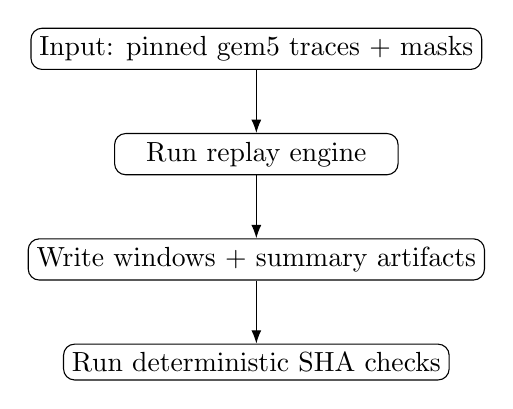
\begin{tikzpicture}[node distance=8mm and 12mm]
\node[box] (a) {Input: pinned gem5 traces + masks};
\node[box, below=of a] (b) {Run replay engine};
\node[box, below=of b] (c) {Write windows + summary artifacts};
\node[box, below=of c] (d) {Run deterministic SHA checks};
\draw[line] (a) -- (b);
\draw[line] (b) -- (c);
\draw[line] (c) -- (d);
\end{tikzpicture}
\caption{gem5 Golden Output Flow}
\end{figure}

\end{document}
